% Vorlage fuer Handouts
% zum Seminar "Diskrete Geometrie und Kombinatorik -- ein topologischer Zugang"
% im WS 2008/09
%
%%%%%%%%%%%%%%%%%%%%%%%%%%%%%%%%%%%%%%%%%%%%%%%%%%%%%%%%%%%%%%%%%%%%%%%%%%%%
% Allgemeine Hinweise
% - Halten Sie den LaTeX-Code so uebersichtlich wie moeglich;
%   (La)TeX-Fehlermeldungen sind oft kryptisch -- in einem ordentlich 
%   strukturierten Quellcode lassen sich Fehler leichter finden und 
%   beseitigen
%
%
%%%%%%%%%%%%%%%%%%%%%%%%%%%%%%%%%%%%%%%%%%%%%%%%%%%%%%%%%%%%%%%%%%%%%%%%%%%%
% Jedes LaTeX-Dokument muss eine \documentclass-Deklaration enthalten
%   Diese sorgt fuer das allgemeine Seiten-Layout, das Aussehen der 
%   Ueberschriften etc.
\documentclass[a4paper,oneside,DIV8,10pt]{scrartcl}
  
  %%%%%%%%%%%%%%%%%%%%%%%%%%%%%%%%%%%%%%%%%%%%%%%%%%%%%%%%%%%%%%%%%%%%%%%%%%
  % Einbinden weiterer Pakete
  %\usepackage{english}    % fuer die deutschen Trennmuster
  % \usepackage{ngerman} % entsprechend fuer die neue Rechtschreibung
  \usepackage[latin1]{inputenc} % falls Sie Umlaute in den Quellen verwenden wollen
  \usepackage{amsmath}   % enthaelt nuetzliche Makros fuer Mathematik
  \usepackage{amsthm}    % fuer Saetze, Definitionen, Beweise, etc.
  \usepackage{relsize}   % fuer \smaller 
  \usepackage{hyperref}  % fuer \url  
  \usepackage{graphicx}  % fuer Grafiken
  \usepackage{listings}  % fuer code
  \usepackage{xcolor}    % fuer Farben
  \usepackage[section]{algorithm} % fuer Algorithmen
  \usepackage{algorithmic}	      % fuer Algorithmen
  
  %%%%%%%%%%%%%%%%%%%%%%%%%%%%%%%%%%%%%%%%%%%%%%%%%%%%%%%%%%%%%%%%%%%%%%%%%%
  % Coding environments
  
  \definecolor{javared}{rgb}{0.6,0,0} % for strings
  \definecolor{javagreen}{rgb}{0.25,0.5,0.35} % comments
  \definecolor{javapurple}{rgb}{0.5,0,0.35} % keywords
  \definecolor{javadocblue}{rgb}{0.25,0.35,0.75} % javadoc
  
  \lstset{language=Java,
  	basicstyle=\ttfamily,
  	keywordstyle=\color{javapurple}\bfseries,
  	stringstyle=\color{javared},
  	commentstyle=\color{javagreen},
  	morecomment=[s][\color{javadocblue}]{/**}{*/},
  	morekeywords={String, Object},
  	otherkeywords={Object},
  	numbers=left,
  	numberstyle=\color{black},
  	stepnumber=1,
  	numbersep=10pt,
  	tabsize=4,
  	showspaces=false,
  	breaklines=true,
  	postbreak=\mbox{\textcolor{red}{$\hookrightarrow$}\space},
  	showstringspaces=false%
  }

  %%%%%%%%%%%%%%%%%%%%%%%%%%%%%%%%%%%%%%%%%%%%%%%%%%%%%%%%%%%%%%%%%%%%%%%%%%
  % Deklaration der Keyboard Tasten
  %Windows
  \usepackage[os=win]{menukeys}
  
  %Mac OS X (symbols)
  %\usepackage[os=mac, mackeys=symbols]{menukeys}
  
  %Mac OS X (text)
  %\usepackage[os=mac, mackeys=text]{menukeys}
  
  %%%%%%%%%%%%%%%%%%%%%%%%%%%%%%%%%%%%%%%%%%%%%%%%%%%%%%%%%%%%%%%%%%%%%%%%%%
  % Deklaration eigener Mathematik-Makros
  \newcommand{\N}{\ensuremath{\mathbf{N}}}   % natuerliche Zahlen
  \newcommand{\Z}{\ensuremath{\mathbf{Z}}}   % ganze Zahlen
  \newcommand{\Q}{\ensuremath{\mathbf{Q}}}   % rationale Zahlen
  \newcommand{\R}{\ensuremath{\mathbf{R}}}   % reelle Zahlen

  %%%%%%%%%%%%%%%%%%%%%%%%%%%%%%%%%%%%%%%%%%%%%%%%%%%%%%%%%%%%%%%%%%%%%%%%%%
  % Deklaration eigener Satz-/Definitions-/Beweisumgebungen mit amsthm
  \newtheorem{satz}{Satz}[section]
  \newtheorem{lemma}[satz]{Lemma}
  \newtheorem{korollar}[satz]{Korollar}
  \theoremstyle{definition}
  \newtheorem{definition}[satz]{Definition}
  \newtheorem{bemerkung}[satz]{Bemerkung}
  \newtheorem{aufgabe}[satz]{Exercise}
  \newenvironment{beweis}%
    {\begin{proof}[Beweis]}
    {\end{proof}}
  \newtheorem{beispiel}[satz]{Beispiel}

  %%%%%%%%%%%%%%%%%%%%%%%%%%%%%%%%%%%%%%%%%%%%%%%%%%%%%%%%%%%%%%%%%%%%%%%%%%
  % Deklaration weiterer Makros
  \renewcommand{\labelitemi}{--}             % aendert die Symbole bei unnumerierten Aufzaehlungen
  \makeatletter                              % Fussnote ohne Symbol
    \def\blfootnote{\xdef\@thefnmark{}\@footnotetext}
  % Titel des Handouts
  %   #1 Name des Vortragenden
  %   #2 email-Adresse 
  %   #3 Datum des Vortrags
  %   #4 Titel des Vortrags
  \newcommand{\handouttitle}[4]
   {\begin{center}
      \Large #4
    \end{center}

    \bigskip

    \noindent
    #1 (\textsf{#2})
    \hfill
    #3%
    \blfootnote{MPS Workshop, AQUA, TU Dortmund}
  
    \noindent
    \rule{\linewidth}{.5pt}

    \bigskip

    \@afterindentfalse\@afterheading
   }
  \makeatother
  \renewcommand{\sectfont}{\normalfont}       % aendert den Font fuer Ueberschriften
  
  \newcommand{\workshoplanguage}[1]{
\includegraphics[height=6px]{graphics/language.png} de.tudo.cs.ls14.aqua.mps.workshop.#1}
  
  \newcommand{\workshoplanguagecreation}[0]{
\includegraphics[height=6px]{graphics/language.png} Language}
  \newcommand{\workshopsolution}[1]{
\includegraphics[height=6px]{graphics/solution.png} de.tudo.cs.ls14.aqua.mps.workshop.#1}
  \newcommand{\workshopmodel}[1]{
\includegraphics[height=6px]{graphics/model.png} #1}
  \newcommand{\workshopnode}[1]{
\includegraphics[height=6px]{graphics/node.png} #1}
  \newcommand{\workshopproject}[0]{
\includegraphics[height=6px]{graphics/project.png} mps-workshop}
  \newcommand{\workshoprun}[0]{
\includegraphics[height=6px]{graphics/run.png} Run 'Node de.tudo.cs.ls14...'}
  \newcommand{\workshopmoduleproperties}[0]{
\includegraphics[height=6px]{graphics/properties.png} Module Properties}
  \newcommand{\workshopruntime}[0]{
\includegraphics[height=6px]{graphics/runtime.png} Runtime}
  \newcommand{\workshopversion}[0]{\menu{
\includegraphics[height=6px]{graphics/version.png} Get from Version Control}}
  \newcommand{\workshopinspector}[0]{
\includegraphics[height=6px]{graphics/inspector.png} Inspector}

%%%%%%%%%%%%%%%%%%%%%%%%%%%%%%%%%%%%%%%%%%%%%%%%%%%%%%%%%%%%%%%%%%%%%%%%%%%%
% Anfang des eigentlichen Dokuments
\begin{document}

  % Titel fuer das Handout -- Sie koennen natuerlich auch selbst etwas entwerfen!
  \handouttitle{Till Schallau}
               {till.schallau@tu-dortmund.de}
               {14.~September~2020}
               {MPS Workshop}

  The following exercise are designed to give you an in-depth understanding for the creation of languages using the MPS language workbench.
  
  \section{Setup - Console}
  
  \begin{enumerate}
  	\item Download the latest version of MPS for your operating system from \\ \url{https://www.jetbrains.com/de-de/mps/download/}
  	\item Clone the \textit{mps-workshop} repository using \\
  	\url{git@aqua-scm.cs.tu-dortmund.de:aqua/mps-workshop.git} or\\
  	\url{https://aqua-scm.cs.tu-dortmund.de/aqua/mps-workshop.git}
  	\item Open the project in MPS with \menu[,]{File, Open}
  	\item When prompted: \menu{migrate} the project
  	\item Right-click on the language \menu[,]{\workshoplanguage{java},Rebuild Language} to make the language available for the sandbox solution
  	\item Right-click on the project \menu[,]{\workshopproject, Rebuild project}
  \end{enumerate}

  \section{Setup - IDE}
  
  \begin{enumerate}
  	\item Download the latest version of MPS for your operating system from \\ \url{https://www.jetbrains.com/de-de/mps/download/}
  	\item Open MPS
  	\item Select \workshopversion
  	\item Enter \url{https://aqua-scm.cs.tu-dortmund.de/aqua/mps-workshop.git} into the \menu{URL} field, select a directory and press \menu{clone}
  	\item When prompted: \menu{migrate} the project
  	\item Right-click on the language \menu[,]{\workshoplanguage{java},Rebuild Language} to make the language available for the sandbox solution
  	\item Right-click on the project \menu[,]{\workshopproject, Rebuild project}
  \end{enumerate}

  \section{MPS Hands-On}
  
  These exercises are designed to give you a feeling of how the projectional editor of MPS is working. For the following tasks, work on the \menu{$\hookrightarrow$  master} branch.
  Navigate to the model \menu{\workshopmodel{sandbox}} under the solution \menu{\workshopsolution{java}} and create a new \menu{\workshopnode{JavaInMPSTest}} node as shown in Figure \ref{fig:sandbox}.
  \begin{figure}[h]
  	\centering
  	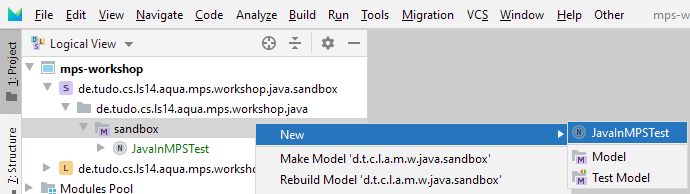
\includegraphics[width=\textwidth]{graphics/sandbox.png}  
  	\caption{Navigation menu for creation of a new \menu{\workshopnode{JavaInMPSTest}} node}
  	\label{fig:sandbox}	
  \end{figure}

  \begin{aufgabe}
  	Implement the code shown in Listing \ref{lst:read-name} in your \menu{\workshopnode{JavaInMPSTest}} node. Notice the change in the predefined code fragment while editing the name of the method. After completion rebuild the model by right-clicking \menu[,]{\workshopmodel{sandbox}, Rebuild model}. When there are no more syntax and compilation errors, run the code by right-clicking onto \menu[,]{\workshopnode{JavaInMPSTest}, \workshoprun}.\\
  	\\
  	\textbf{Note:} You can check the generated code by right-clicking onto the editor and select \menu{Preview Generated Text}.
  	
  	\begin{lstlisting}[language=Java,caption={Java code to read a line from the console and print the result}, captionpos=b, label={lst:read-name}]
public static void readLine(){
	String name = "";
	try{
		System.out.println("Hello! Please enter your name.");
		BufferedReader br = new BufferedReader(new InputStreamReader(System.in));
		name = br.readLine();
		System.out.println("Hello " + name);
	} catch(Exception e){
		throw e;
	}
}
  		\end{lstlisting}
  \label{alg:read-name}
  \end{aufgabe}

  \begin{aufgabe}
  	Be creative! Add a new \menu{\workshopnode{JavaInMPSTest}} node and add your own code.\\
  	\\
  	\textbf{Note:} If your desired package does not exist in your current context, you can add \textit{Accessories Models} by right-clicking the language \menu[,]{\workshoplanguage{java}, \workshopmoduleproperties}. Navigate to \menu[,]{\workshopruntime, Accessories Models} and add the required models using the \menu{+} button, e.g. \menu{\texttt{\workshopmodel{java.time@java\_stub}}}. You have to rebuild the language \menu[,]{\workshoplanguage{java}, Rebuild Language} to apply your change.
  \end{aufgabe}

	\section{Expressions}
	
	This section is designed to show you the most important core aspects of MPS. Each sub-exercise can be pulled from their respective branch, such that each task can be done based on a shared code base.
	
	\begin{aufgabe}
		Create a new language named \\
		\texttt{de.tudo.cs.ls14.aqua.mps.workshop.expressions} by right-clicking onto\\ \menu[,]{\workshopproject, New, \workshoplanguagecreation}. Check the \menu{Create Sandbox Solution} in the process. You have to build the language \menu[,]{\workshoplanguage{expressions}, Rebuild Language} to remove errors.
	\end{aufgabe}

	\begin{aufgabe}
		Translate the BNF of Table \ref{table:bnf} into concepts. You may use abstract concepts to simplify the task and add internal structure.\\
		Give each concept a meaningful \textbf{name} and \textbf{short description}.
		\begin{table}
			\begin{tabular}{ l r l }
				Class & ::= & Function*\\
				%
				\\
				%
				Function & ::= & ID = AExp\\
				& $|$ & ID = BExp \\
				%
				\\
				%
				AExp & ::= & AExp $+$ AExp\\
					 & $|$ & AExp $-$ AExp\\
					 & $|$ & AExp $*$ AExp\\
					 & $|$ & AExp $/$ AExp\\
					 & $|$ & INT\\
					 & $|$ & ID //variable\\
			\end{tabular}
			\begin{tabular}{ l r l }
			BExp & ::= & BExp $\&\&$ BExp \\
			& $|$ & BExp $||$ BExp\\
			& $|$ & AExp $==$ AExp\\
			& $|$ & AExp $!=$ AExp\\
			& $|$ & AExp $\geq$ AExp\\
			& $|$ & AExp $>$ AExp\\
			& $|$ & AExp $\leq$ AExp\\
			& $|$ & AExp $<$ Aexp\\
			& $|$ & True \\
			& $|$ & False \\
			& $|$ & ID //variable\\
		\end{tabular}
	\caption{BNF of arithmetic and boolean expressions}
	\label{table:bnf}
		\end{table}
	\end{aufgabe}

	For the next exercise you can checkout the branch \menu{$\hookrightarrow$  expression-0-concepts} to work with the shared solution, or work with your own concepts.

	\begin{aufgabe}
		Add editors for your concepts, such that the order of operations is clearly visible.\\
		\\
		\textbf{Note:} For some visual modifications you may need the \menu{\workshopinspector}. To show it, click on the respective button in the lower right corner of your IDE.
	\end{aufgabe}

	Intermediate solution: \menu{$\hookrightarrow$ expression-1-editors}
	
	\begin{aufgabe}
		Add intentions for the \texttt{and}- and \texttt{or}-Expression which transforms a given node into the other and vice versa.
	\end{aufgabe}

	Intermediate solution: \menu{$\hookrightarrow$ expression-2-intentions}
	
	\begin{aufgabe}
	Add checks to ensure that each function name is unique. Add checks to ensure that each variable is unique for each function.
	\end{aufgabe}

	Intermediate solution: \menu{$\hookrightarrow$ expression-3-checks}
	
	\begin{aufgabe}
	Add transformations that automatically append a node into the AST after typing a specific keyword. Write transformations for the \texttt{and}- and \texttt{or}-Expression for both directions (left and right).
	\end{aufgabe}

	Intermediate solution: \menu{$\hookrightarrow$ expression-4-transformations}
	
	\begin{aufgabe}
		Add generators for at least one of \texttt{AExp} or \texttt{BExp}. Your code construct for the expression \texttt{x >= 2} should look like the following  Listing \ref{lst:gen}.
	\end{aufgabe}

	The final solution with all steps can be found under \menu{$\hookrightarrow$ expression-5-generations}
	
	\newpage
		
		\begin{lstlisting}[language=Java,caption={Generated Java code that parses the variables and returns the result of the defined expression}, captionpos=b, label={lst:gen}]
package de.tudo.cs.ls14.aqua.mps.workshop.expressions.sandbox;

/*Generated by MPS */

import java.io.BufferedReader;
import java.io.InputStreamReader;

public class ExpressionTest {
	public static void main(String[] args) {
		test();
	}
	public static void test() {
		BufferedReader reader = new BufferedReader(new InputStreamReader(System.in));
		int x = -1;
		
		try {
			System.out.println("Please enter value for int-variable " + "x");
			String line = reader.readLine();
			x = Integer.parseInt(line);
		} catch (Exception e) {
		}
		boolean z = (x >= 2);
		System.out.println("The result of your function test is: " + z);
	}
}
		\end{lstlisting}


%%%%%%%%%%%%%%%%%%%%%%%%%%%%%%%%%%%%%%%%%%%%%%%%%%%%%%%%%%%%%%%%%%%%%%%%%%%%
% Ende des Dokuments -- alles, was nach dieser Zeile steht, wird 
% von LaTeX ignoriert!
\end{document}